% 13:52 06/04/2023
\chapter{Technology Review}
% This chapter is the literature review part of the dissertation
% and should be tightly coupled to the context and objective from the introduction.
% A thorough Technology Review proves that you researched what you were doing!

This chapter provides a technical review of the technologies used in the platform.

Detailing the reasoning behind selecting these specific technologies
and how they contribute to accomplishing the objectives laid out in the introduction.

Also covering technologies specifically related to malware detection,
these include Sandboxie and Process Monitor,
and widely accepted standards like JSON for transmitting data over networks.

For the server section, it shows how the use of tooling like Docker
can help with the creation of reproducible environments.

First, there will be a discussion on the technologies that are general
to all the sub-projects,
and what was used to create the chatbot for the promotional page.
Then the technologies that were used in each sub-project.

\section{JSON}
In the platform, there will be multiple computers that receive and transmit data.
There needs to be an agreed-upon format between these
computers in which the data is encoded.
The format must support dictionaries and lists to express data structures.

JSON has been chosen for this because the browser has
native support for encoding and decoding JSON,
Python supports it through the \texttt{json} module,
and Racket also has it in its standard library.
JSON stands for JavaScript Object Notation,
a widely-used format for transmitting and storing data. \\

It provides a standardised way of serialising complex data structures or collections,
making it easy to transfer data between different systems.
JSON can be used to represent a wide range of data types,
including lists, dictionaries, and primitive types such as numbers and strings. \cite{ECMA-404}

The standard document for JSON cited above
provides developers with a specification to easily
implement JSON encoding and decoding in their language.
Also, its simplicity has made it popular amongst developers. \\

Below you will find an example of JSON being used in the browser to encode a dictionary:

\begin{lstlisting}[language=Java]
const myData = {"1": 2, 3: 4.0};
console.log(JSON.stringify(myData));
\end{lstlisting}

And this is an example of it being used in Python, using the \texttt{json} module.

\begin{lstlisting}[language=Python]
import json

my_data = {"1": 2, 3: 4.0}
print(json.dumps(my_data))
\end{lstlisting}

\section{Python}
Python \cite{python} is an interpreted, high-level, general-purpose programming language.
I chose to use Python because I wanted to use the same language for the client and the server.
When I serialised data on the client side, I could use the same
 library, to deserialise it on the server.

Python is also a very simple language and can be run without compliation,
this allowed me to quickly test code, without having to compile it every time. \\

Python comes with a package manager called \texttt{pip},
which is accessible on all operating systems,
this allows me to easily install dependencies required by the server.
Python is less verbose than languages like Java,
allowing you to get a lot done with a small amount of code.

\section{GPT-3.5}
In recent months, the popularity of large language models has exploded,
primarily due to the advent of ChatGPT.

OpenAI, the creator of GPT, provides an
API to their GPT-3.5 model \cite{openai}.
This model has been trained on a large corpus of text from the internet
and can make predictions based on inputs to the model. \\

Currently, this technology represents the state of the art in
artificial intelligence and
OpenAI's API makes it freely available to anyone.

To promote the platform, I have created a promotional page on
GitHub pages and added a bot (CaladiumBot),
that can answer questions about it.
I fetch the latest version of the \texttt{README.md} file for
this project, feed it into the OpenAI model as an initial prompt,
and then used it to answer user's questions about the platform. \\

OpenAI provides a module for Python,
below you will find a minimal example of how I'm using it.
The full implementation can be found in \texttt{bot/\_\_main\_\_.py}.

\begin{lstlisting}
import openai # Set OpenAI API key as environmental variable
openai.api_key = os.environ.get("OPENAI_API_KEY", None)

initial_prompt = """
You are CaladiumBot, you will answer questions
about the README listed below:
"""
# Append the README here

prompt = [{"role": "system", "content": initial_prompt}]
question = input("Your question: ")
prompt += [{"role": "user", "content": question}]

# This will output the GPT response to the command-line
print(openai.ChatCompletion.create(model="gpt-3.5-turbo", \
        messages=prompt).choices[0].message.content)
\end{lstlisting}

\section{Technology in the Client Side}
As stated in the objectives, there will be a native GUI application,
this will be a Windows application so it will not run in the browser,
the application will be written in Python,
so I am using Python-specific libraries to develop it.

\subsection{PyInstaller}
A common reason why more people don't opt to use Python over a
native language such as C/C++ is the fact you require Python
to run the code.
Some users of a particular software might
want to be able to run the software without having to install Python first. \\

PyInstaller \cite{pyinstaller} is a module for Python that allows you to bundle your
Python code with a Python interpreter, allowing it to be run on any computer
that doesn't have Python installed.
This allows your software to be self-contained and portable,
users don't have to install Python on their computers to run your software.

As shown in the documentation you can easily
convert a Python project into a bundle. \cite{pyinstaller}
Pass the main file location of the Python project into PyInstaller: \\
\texttt{pyinstaller \_\_main\_\_.py}

\subsection{Tkinter}
Tkinter \cite{tkinter} is the standard GUI library for Python,
It is also cross-platform, allowing the client to run on Windows, Linux and macOS.
It is stable and mature, with a plethora of documentation to be found on the internet. \\

Tkinter makes it very easy to create a GUI with a small amount of code,
which allowed me to quickly build a prototype of the GUI application.
The library features many GUI components including buttons, labels and input boxes,
these are important for creating a native GUI application experience for Windows.

I will give an example below, of creating a simple GUI window.

\begin{lstlisting}
import tkinter

# Creating the main window object
main_window = tkinter.Tk()
# Main loop of execution, polling for updates
main_window.mainloop()
\end{lstlisting}

Running this code will result in the window shown above.
This serves as a stark reminder of the power of Tkinter
and its ability to create interfaces quickly.

\begin{figure}[h!]
    \centering
    \label{image:tkinterWindowScreenshot}
    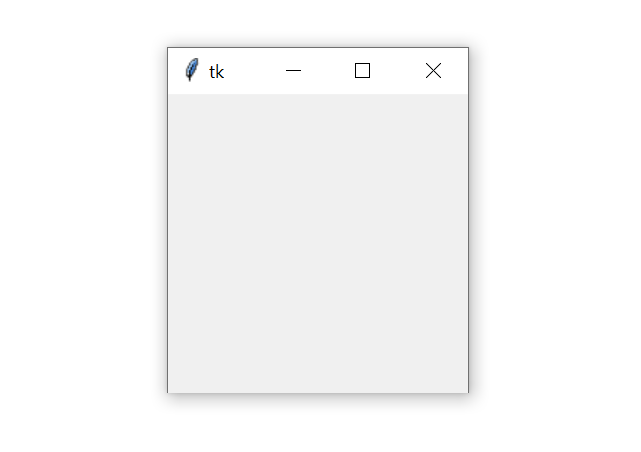
\includegraphics[width=0.65\textwidth]{images/screenshots/tkinter}
    \caption{Tkinter Window Screenshot}
\end{figure}

\subsection{tkthread}
In Tkinter applications, there exists an infinite \textbf{mainloop}
(as seen in the example above)
that runs until the user closes the application.

Whenever a user clicks a button,
it triggers an event that calls the corresponding callback function
that was specified during the button's creation.

As this call blocks the \textbf{mainloop}'s execution,
a function that takes a long time to complete can cause the GUI to freeze,
causing the program to become unresponsive.

While a naive solution might involve threading,
this approach requires thread synchronisation and can lead to race conditions
and phantom threads, leading to even more problems than it fixes.

Instead, tkthread \cite{tkthread} provides a more elegant solution.
tkthread is a third-party module for Python,
that is non-affiliated with the developers of Tkinter.

In the example below, I'm showing how you can use tkthread to patch
Tkinter to allow async operations,
when the button is pressed it will spawn an async thread,
and every so often it will give the
UI a certain amount of time to draw itself.

This results in much cleaner code,
and avoid complexities like using threading,
instead running callback functions asynchronously.

\begin{lstlisting}
import tkthread
# Patch tkinter to allow async operations
tkthread.patch()

import tkinter

main_window = tkinter.Tk()

def button_callback():
  # Spawn new thread
  @tkthread.main(main_window)
  def my_thread():
    while True:
      print("This won't block the GUI")
      
      main_window.update() # Allow UI to update
      main_window.after(1000)

# Create new button, that will call the function above
my_button = tkinter.Button(main_window,
    text="Test Button", command=button_callback)
my_button.pack()

main_window.mainloop()
\end{lstlisting}

\subsection{JavaScript}
JavaScript was used in the dashboard to add dynamicity,
it is used to fetch data from the server using the RESTful API endpoints
and display it on the screen.

I wanted to take full advantage of all the new
JavaScript features that were brought in
recent years, these include the ability to have classes and
the new \texttt{fetch} function as an alternative to
setting up the XMLHttpRequest object.

The 6th edition of the ECMAScript standard \cite{ES6} (JavaScript standard) 
introduced the \texttt{class} keyword for creating classes,
before this developers had to create classes through prototypes.

Classes are important in the dashboard because the list page classes
all inherit from a common superclass allowing them to share code.

\begin{lstlisting}[language=Java]
class Page {
    int x;

    constructor(newX) {
        this.x = x;
    }

    getX() {
        return this.x;
    }

    setX(newX) {
        this.x = newX;
    }
}
\end{lstlisting}

Here is the legacy syntax, as can be seen, it is quite verbose,
and it isn't encapsulated in the class like above.

\begin{lstlisting}[language=Java]
function Page(newX) {
    this.x = newX;
}

Page.prototype.getX = function() {
    return this.x
}

Page.prototype.setX = function(newX) {
    this.x = newX;
}
\end{lstlisting}

Another addition of the ECMAScript 2015 standard is the \texttt{fetch} function,
prior to this, you'd have to use the \texttt{XMLHttpRequest} object,
this is important in Caladium because it allows the dashboard to
request data from the server through the RESTful APIs.

Below you can find an example of the \texttt{fetch}
being used in the dashboard,
\texttt{fetch} accepts a number of parameters including the resource path,
the HTTP headers, in this case, the \textbf{Authorisation}
token and a body containing the data being sent to the server.

\begin{lstlisting}
const caladiumFetchParameters = {
    method: method, headers:
        {"Authorisation": localStorage["Authorisation"]},
    body: body ? JSON.stringify(body) : undefined
};
const resp = await fetch(path, caladiumFetchParameters);
// Returns when the response is resolved
return await resp.json();
\end{lstlisting}

\section{Technology in the Server}
The server is the main component of the platform,
bridging communication between the clients and the sandbox instances, 
and providing RESTful APIs for the clients to interact with it.

The server needs to be able to persist data for the administrators, 
which is stored in CouchDB. Since the server is written in Python,
it requires the pycouchdb library to communicate with the DB instance.

I have also created a \texttt{Dockerfile} for Docker
that enables people to easily replicate the required
environment for running the server.

\subsection{Flask}
I needed a way for the dashboard and the clients to be
able to communicate with the server
I decided to use Flask to create the HTTP endpoints.

Flask \cite{flask} is a micro web framework written in Python.
It is classified as a micro-framework because it does
not require any extra tools or libraries.
This allowed me to create the HTTP endpoints for the RESTful API without
having to worry about the underlying HTTP server.

The simplicity of Flask allows for quick prototyping,
which speeds up the development cycle.
Many accept Flask as the de facto framework
for creating web applications in Python.
This led me to choose Flask as the framework for the server component.

Below you will find some example code to create a Flask server,
with a GET endpoint that returns the text "\texttt{Index Page}" on request. \\ \\

\begin{lstlisting}[language=Python]
import flask

app = flask.Flask(__name__)

@app.get("/")
def root_page(): return "Index Page"

app.run()
\end{lstlisting}

When you run this code, it will spawn an instance of Flask,
listing the IP address of the server,
this usually being \texttt{http://127.0.0.1:5000}.

Below you can find a screenshot of the
\texttt{/} route in the browser.


\begin{figure}[h!]
    \centering
    \label{image:dockerDiagram}
    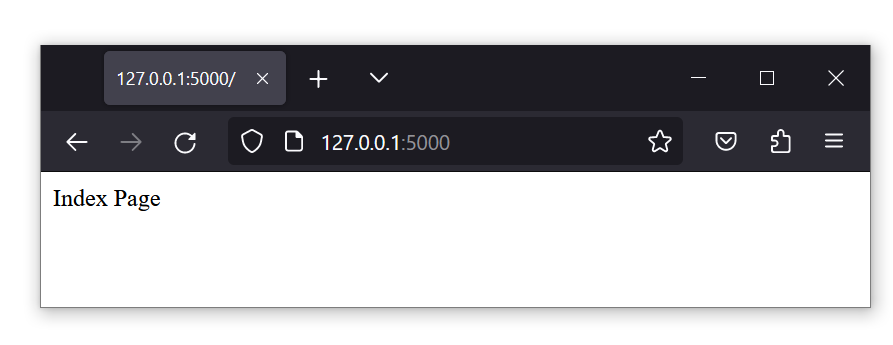
\includegraphics[width=0.85\textwidth]{images/screenshots/flask_server_screenshot}
    \caption{Flask Server in Browser Screenshot}
\end{figure}

\subsection{Representational State Transfer}
I am using REST to model the HTTP endpoints for the server,
REST was first described in Roy Thomas Fielding's dissertation \cite{REST}
as a way of architecting APIs in a stateless manner to
access resources over a network connection.

REST is a set of best practices for how systems should interact with one another.
It promotes scalability and allows for caching of resources.

HTTP methods can be used to perform actions on a resource.
For example, the \textbf{GET} method can be used to fetch data,
which can also be cached.
The \textbf{DELETE} method can be used to delete a record by its ID. \\ \\ \\ \\ \\

For example, if there existed a set of endpoints that
performed actions on a database of tasks. \\

\textbf{GET} \texttt{/api/tasks} \\
Would return a JSON array, containing all the tasks.

\textbf{POST} \texttt{/api/tasks} \\
Would be used to create a new task,
and you'd pass in the new task through the HTTP body.

\textbf{DELETE} \texttt{/api/tasks/0001} \\
Would be used to delete a task by its ID,
in this case, it would be the task with ID \texttt{0001}.

\subsection{CouchDB}
CouchDB is a document-oriented NoSQL database. \cite{couchdb}
An important feature of any platform is the ability to persist data.

In my case, I am using CouchDB to store the records for the
\textbf{clients}, \textbf{patterns}, \textbf{tasks} and \textbf{workers} tables.

I find NoSQL quite convenient compared to SQL databases,
because I don't have to write out the queries,
and NoSQL allows you to easily append JSON objects to the tables.

I went with CouchDB because of the simplistic nature of
a document database is appealing,
allowing me to spend more time on more complex features.
CouchDB is also scalable, allowing many instances of it,
allowing it to increase with more users.

CouchDB provides an HTTP/JSON API, allowing any programming language
with an HTTP library to interface with the DB instance.

\subsection{pycouchdb}
Python alone isn't able to communicate with the CouchDB instance,
and requires a library, in this case, it's \textbf{pycouchdb}.

pycouchdb provides an API for developers to easily interface with
CouchDB, without having to write the HTTP requests to do so.

The example below shows how to use pycouchdb,
to create a table called "tasks" and add a record.

\begin{lstlisting}
import pycouchdb

# Connect to the DB using the connection str in the env variable
couchdb_server = pycouchdb.Server(os.environ["COUCHDB_CONNECTION_STR"])

# Create the table, and create a new record with the dictionary
tasks_table = couchdb_server.create("tasks")
tasks_table.save({"name": "task"})
\end{lstlisting}


\subsection{Docker}
Docker is a tool used by developers to create reproducible environments. \cite{docker}
Meaning you can run your software on different computers,
and it would have the exact same stuff installed.

Most open-source projects come with a \texttt{Dockerfile}, it provides
users interested in setting up the project on their own computer,
with the same environment, the developers used.

\begin{figure}[h!]
    \centering
    \label{image:dockerDiagram}
    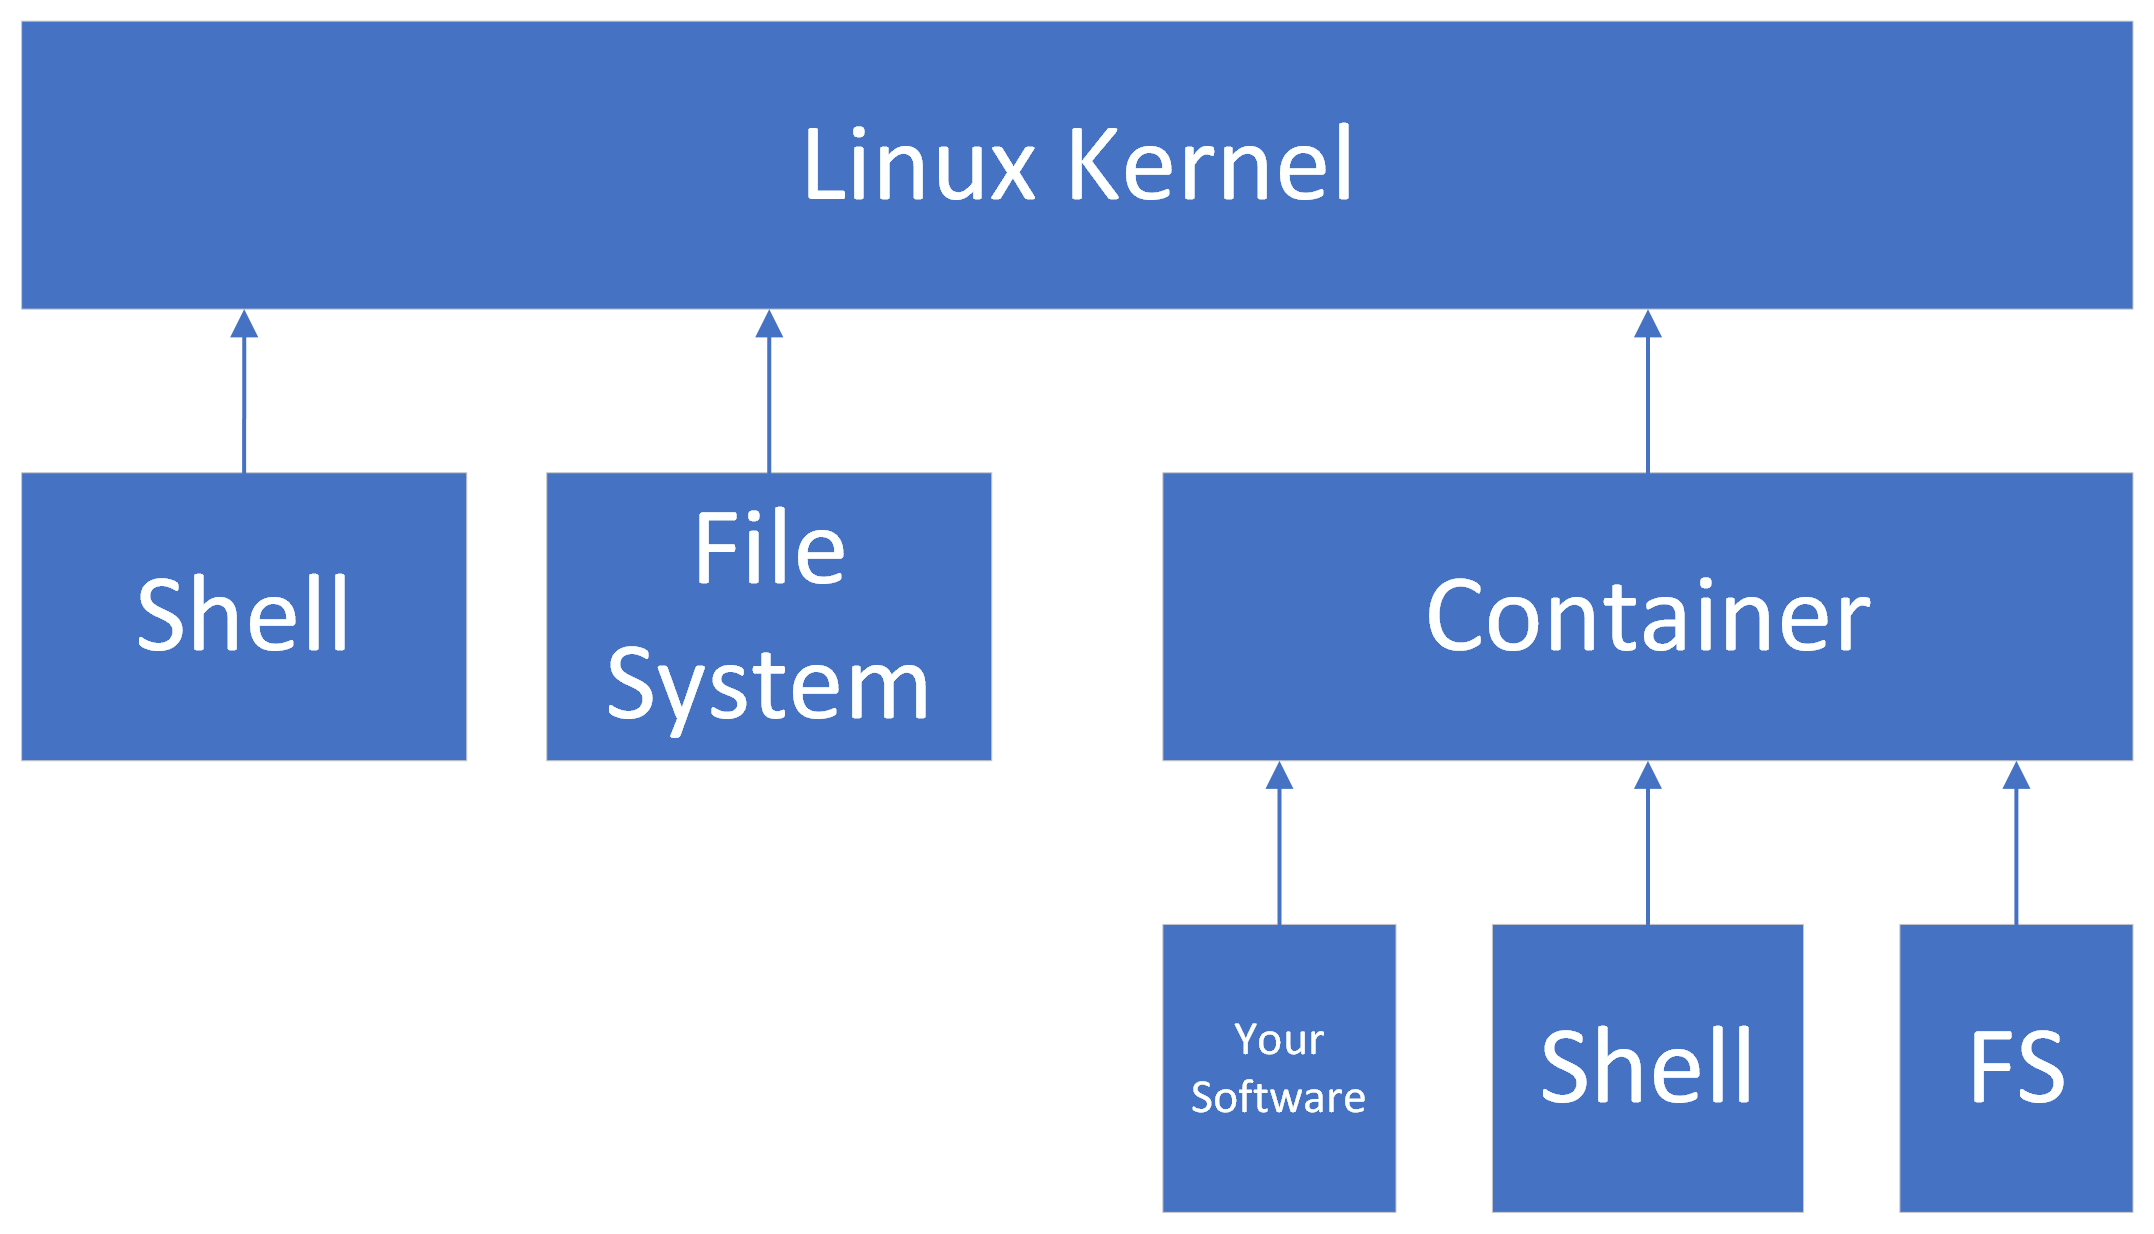
\includegraphics[width=0.65\textwidth]{images/diagrams/docker}
    \caption{Docker Diagram}
\end{figure}

In the diagram above, you can see the host operating system
on the left and the container on the right.
Everything still goes through the Linux kernel,
unlike a virtual machine that runs an entire operating system in isolation. \\

The container has its own file system,
which contains all the utilities for that operating system.
In this project, I'm using Debian for the container,
and the host is using Ubuntu.
Your software running in the container is unable to see
what's going on in other containers or the host operating system
due to isolation features offered by the kernel.

The \texttt{Dockerfile} contains instructions for the Docker daemon,
this is a program that must be installed
on a computer you want to use Docker on.
You must then build containers using this file,
you can have multiple containers on one machine,
this is equivalent to having different computers with different Linux distributions.

You must then run these containers to
execute the code of the project.
These containers are isolated from the main system,
and cannot edit files on the host system.
I am using Docker to make it easy to test my project on different machines,
allowing me to delete them easily,
and not have to actually install the dependencies on my main host system.

The \texttt{Dockerfile} I am using in my project can be found here:
\texttt{server/Dockerfile}

The Dockerfile begins by instructing the daemon,
to install the Linux Debian bullseye version.
Then refresh the apt-get package manager,
and install Python and the Python pip package manager.
Installs the required Python modules,
and copies the server files into the \texttt{/caladium} directory.

Then when you execute the container,
it runs the \texttt{\_\_main\_\_.py} on port 8080.

\begin{lstlisting}
FROM debian:bullseye

RUN apt-get update -y
RUN apt-get install python3 python3-pip -y

RUN python3 -m pip install flask pycouchdb requests

WORKDIR /caladium

COPY src/ /caladium

ENTRYPOINT ["python3"]
CMD ["__main__.py", "8080"]
\end{lstlisting}

\subsection{unittest}
\textbf{Unittest} is a module that comes bundled with Python
and allows you to create test cases for your code \cite{unittest}.
It takes inspiration from JUnit, which is a popular Java testing framework.

To create a test case, you must create a class
that inherits the \texttt{unittest.TestCase} class.
Each of the test methods in your test case class
must be prefixed with \texttt{test\_}.
In each of the methods, you call \texttt{self.assertEquals}
and check if the output of the function in question returns the intended output.

This allowed me to create tests for the endpoints and check
if they returned their intended outputs.

\section{Technology in the Analysis Side}
In this section, I will be discussing the technology that
facilitates the scanning of files and the Racket programming language
I used to write the main part of the scanning side.

\subsection{Sandboxie}
Sandboxie \cite{sandboxie} is a tool for Microsoft Windows designed for sandboxing,
it provides a secure environment to run potentially malicious software.

Typical Windows applications, for example, your browsers like Chrome or Firefox,
never actually have direct access to your system's hard drive.
Instead, they have to go through the operating system, specifically the kernel,
to gain access. If the requesting applications lack the required permissions
the operating system can reject the request.

Sandboxie works by intercepting the system calls made by these applications,
it then identifies the application that made the request,
if the process is currently running under Sandboxie,
it will fake a response, making the application think it was successful,
allowing it to think it has more power than it actually has.

The main purpose of using Sandboxie is to provide an
easy to use isolation software for users, to run software
without worrying about it harming the system.

Sandboxie provides plenty of documentation on how to use the software, on its website,
and the utilities that come with the software come with command-line parameters,
allowing programmers to interface with it programmatically.

Below you will find an example command of how to run the Windows
\textbf{notepad} in a sandbox:

\begin{lstlisting}
"%ProgramFiles%\Sandboxie\Start.exe" notepad.exe
\end{lstlisting}

\begin{figure}[h!]
    \centering
    \label{image:sandboxieScreenshot}
    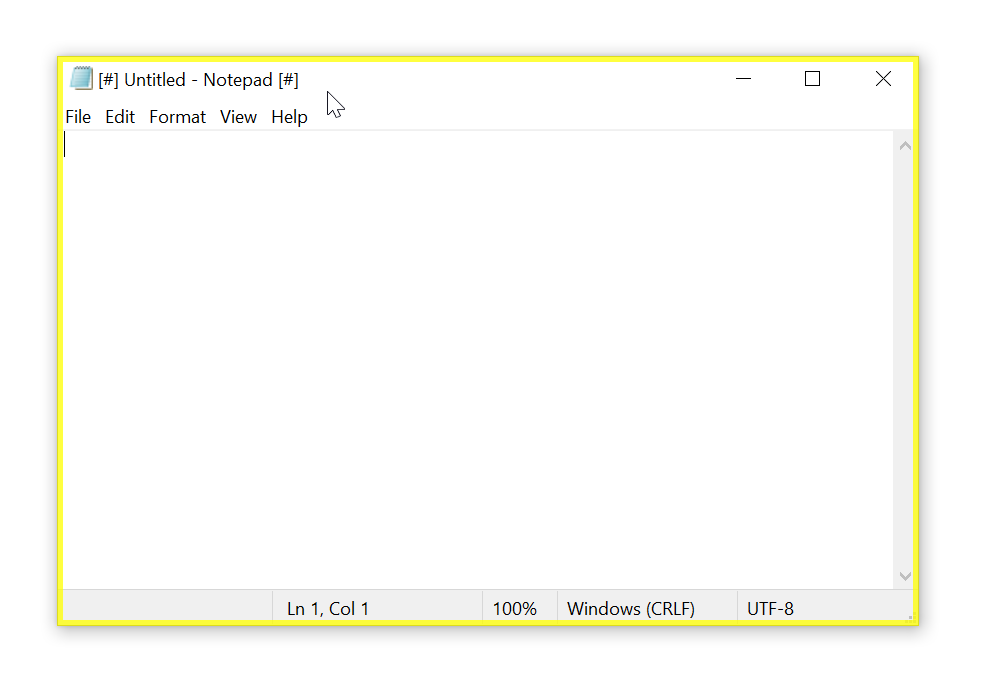
\includegraphics[width=0.75\textwidth]{images/screenshots/sandboxie}
    \caption{Notepad Running in Sandboxie Screenshot}
\end{figure}

Above you can find a screenshot
of \texttt{notepad.exe} running in Sandboxie,
notice how it adds a yellow border to windows
indicating they are being sandboxed.

\subsection{Process Monitor}
Process Monitor is a system monitoring program that allows you to log system calls.
It was created by Microsoft to serve as a monitoring tool, giving power users
the ability to see what exactly every process on their machine is doing,
it produces a log, of all the actions performed and the name of the process that did it.

I needed a way of finding out what the malware is doing,
so I decided to use Process Monitor to log system calls.
I originally was thinking of creating a driver to log system calls,
but I decided to use Process Monitor instead,
to avoid reinventing the wheel.

As described by my research in the methodology chapter,
Process Monitor features command-line parameters
allowing it to be programmatically controlled by your code.

\begin{figure}[h!]
    \centering
    \label{image:procmonScreenshot}
    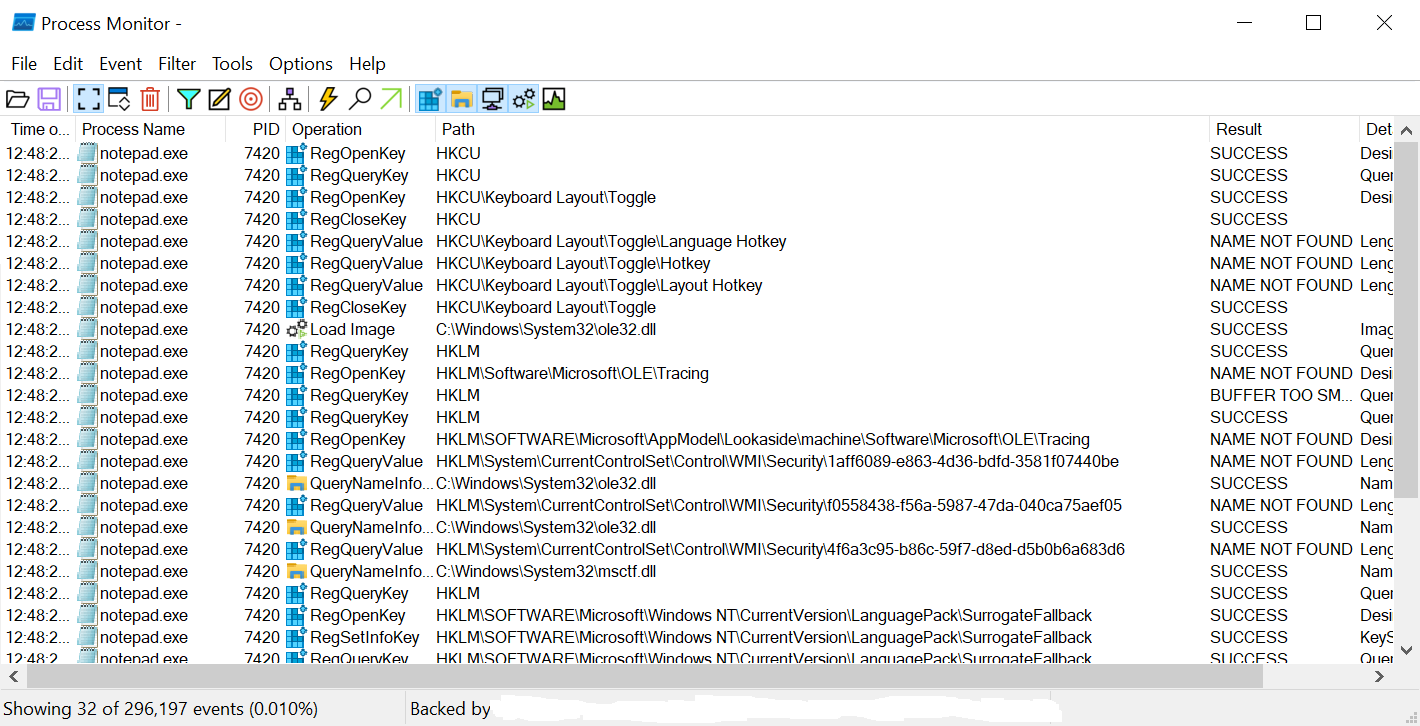
\includegraphics[width=1\textwidth]{images/screenshots/process_monitor}
    \caption{Process Monitor Screenshot}
\end{figure}

Above, you can find a screenshot of Process Monitor
logging the system calls of \texttt{notepad.exe}.
Each line reports the operation it performed,
which can be reading/writing files or creating registry keys.

\bigbreak
\bigbreak
\bigbreak

\subsection{Racket}
Racket is a functional programming language. \cite{racket}
I decided to program the main part of the analysis in Racket
because I've used a lot of Python in other components and
wanted to use a different programming language.

Functional programming languages encourage immutability,
this means once variables are set a value, then they can't be updated.
If you want to update a variable then you must create a new one with
the changes.

Racket is based on Lisp, which means List Processor,
nearly everything in Racket is a list,
Lisp stems from lambda calculus which is an area
of mathematics for expressing computational models. \\

Below you can find a function written in Racket that adds two numbers,
the list begins with "define", the seconds parameter is the function name and arguments,
and finally, the body of the function.

\begin{lstlisting}
(define (add x y)
    (+ x y))
\end{lstlisting}

Racket comes with a plethora of documentation which can be found on its website.

\subsection{ClamAV}
ClamAV is an open-source anti-malware solution that
supports Windows, macOS and Linux. \cite{clamav}
This is the software I'm using to perform my static analysis.

Most anti-malware software are paid and/or closed source,
but ClamAV is the exception, on its website, you can find a rich set of documentation. \\

It comes with a number of command-line utilities.
In my case, I was concerned with the \textbf{clamscan} command, and its parameters.
Most anti-malware solutions don't provide low-level access to their software
requiring you to use their menuing because that's who their target audience is.

ClamAV is targeted at power users,
giving them the ability to modify the source code,
and being able to add their own malware definitions.

I had some difficulties with setting up ClamAV on Windows,
ClamAV is mostly targeted towards Linux users,
but I found a modified distribution of ClamAV optimised for Windows
called ClamWin.

ClamWin periodically downloads the latest malware
definitions from its website,
this all happens automatically. \\

Below you will find a screenshot of the use of the \texttt{clamscan} program,
which comes bundled with ClamAV, to scan the \texttt{notepad.exe} file.
Its malicious status is denoted by \texttt{Infected files: 0}.
This shows how easy it is to use ClamAV programmatically to statically scan files.

\begin{figure}[h!]
    \centering
    \label{image:clamscanScreenshot}
    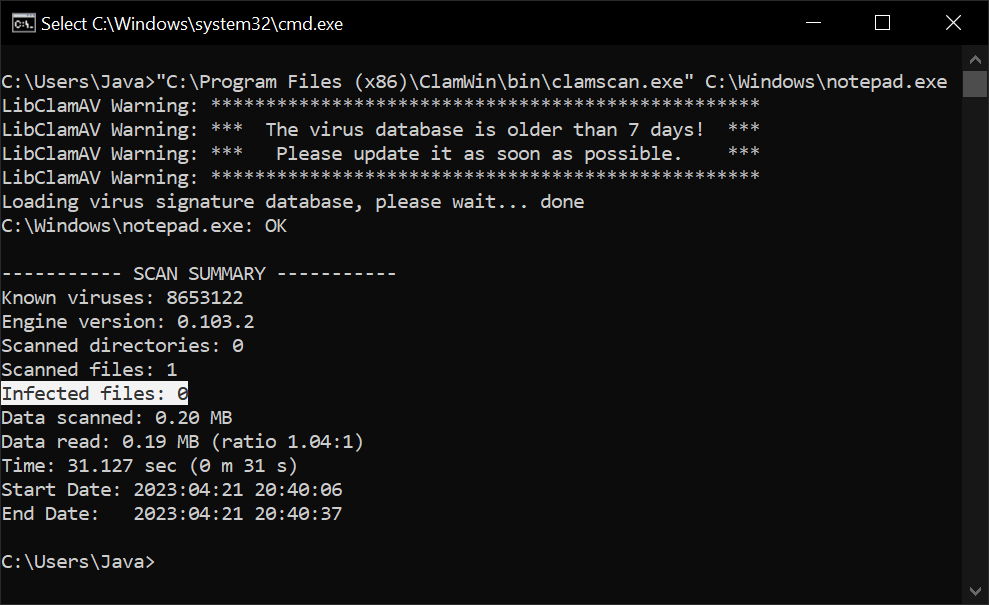
\includegraphics[width=1\textwidth]{images/screenshots/clamscan}
    \caption{ClamAV Scan Screenshot}
\end{figure}
